\documentclass[border=1pt]{standalone}
% Shared preamble for the PixelRoot figures: Times text and math to match
% IEEEtran; every figure is drawn at its printed size (no scaling in the paper).
\usepackage[T1]{fontenc}
\usepackage{mathptmx}
\usepackage{amsmath}
\usepackage{xcolor}
\usepackage{tikz}
\usetikzlibrary{arrows.meta,positioning,calc,fit,backgrounds,decorations.pathreplacing,shapes.geometric}
\definecolor{ink}{HTML}{1B2838}
\definecolor{acc}{HTML}{1F5FBF}
\definecolor{grn}{HTML}{1E7B3A}
\definecolor{red}{HTML}{B3261E}
\definecolor{amb}{HTML}{9A6B00}
\definecolor{cu}{HTML}{B87333}
\tikzset{
  >={Stealth[length=1.6mm,width=1.2mm]},
  every picture/.style={line width=0.6pt, font=\footnotesize, color=ink},
  blk/.style={draw=ink, rounded corners=1.5pt, align=center, inner sep=2.5pt,
    minimum height=9mm, fill=white},
  note/.style={font=\scriptsize, align=left, text=ink!80},
}

\begin{document}
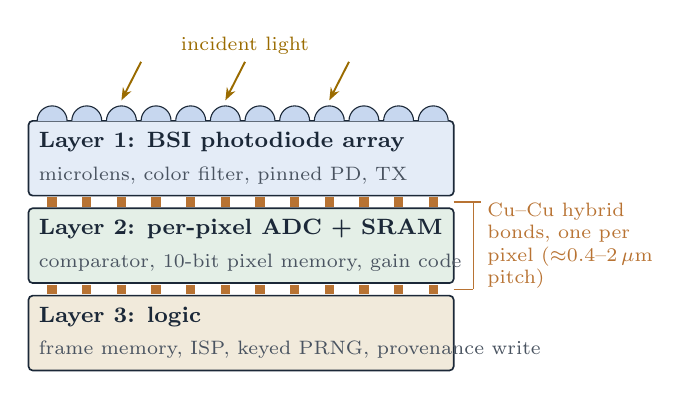
\begin{tikzpicture}
\def\W{5.4}
\def\H{0.95}
\def\gap{0.16}
% layers, top to bottom
\foreach \i/\fill/\title/\sub in {
  0/acc!12/{Layer 1: BSI photodiode array}/{microlens, color filter, pinned PD, TX},
  1/grn!12/{Layer 2: per-pixel ADC + SRAM}/{comparator, 10-bit pixel memory, gain code},
  2/amb!14/{Layer 3: logic}/{frame memory, ISP, keyed PRNG, provenance write}} {
  \pgfmathsetmacro{\y}{-\i*(\H+\gap)}
  \draw[fill=\fill, rounded corners=1.5pt] (0,\y) rectangle (\W,\y-\H);
  \node[anchor=north west, font=\footnotesize\bfseries, inner sep=0pt] at (0.12,\y-0.13) {\title};
  \node[anchor=south west, font=\scriptsize, text=ink!80, inner sep=0pt] at (0.12,\y-\H+0.14) {\sub};
}
% Cu-Cu hybrid bond pads at the two interfaces
\foreach \i in {1,2} {
  \pgfmathsetmacro{\y}{-\i*(\H+\gap)+\gap/2}
  \foreach \k in {0,...,11} {
    \fill[cu] (0.3+\k*0.44-0.06,\y-0.06) rectangle ++(0.12,0.12);
  }
}
% microlenses
\foreach \k in {0,...,11} {
  \draw[fill=acc!25, line width=0.4pt] (0.3+\k*0.44-0.19,0) arc (180:0:0.19);
}
% incident light
\foreach \k in {2,5,8} {
  \draw[->, amb, line width=0.7pt] (0.3+\k*0.44+0.25,0.75) -- (0.3+\k*0.44,0.26);
}
\node[anchor=south, text=amb, font=\scriptsize] at (0.3+5*0.44+0.25,0.72) {incident light};
% annotations
\coordinate (b1) at (\W,-\H-\gap/2);
\coordinate (b2) at (\W,-2*\H-1.5*\gap);
\draw[cu, line width=0.5pt] (b1) -- ++(0.25,0) |- ++(0.1,0) coordinate (n1);
\draw[cu, line width=0.5pt] (b2) -- ++(0.25,0) -- ++(0,0) coordinate (n2);
\draw[cu, line width=0.5pt] ($(b1)+(0.25,0)$) -- ($(b2)+(0.25,0)$);
\node[anchor=west, align=left, text=cu, font=\scriptsize] at ($(b1)!0.5!(b2)+(0.3,0)$)
  {Cu--Cu hybrid\\bonds, one per\\pixel ($\approx$0.4--2\,$\mu$m\\pitch)};
\end{tikzpicture}
\end{document}
